Nuclear forensics comprises a large part of an investigation into a nuclear
incident, such as interdicted nuclear material or the detonation of a weapon
containing radioactive components.  The forensics portion of the investigation
encompasses both the analysis of nuclear material and/or related paraphernalia
as well as the interpretation of these results to establish nuclear material
provenance. The former has many technical aspects, relying on a range of
nuclear science and chemistry.  The latter involves intelligence and political
considerations of the material analyses for attribution. This review will only
consider the technical portion of the nuclear forensics workflow.

First discussed are the types of forensic investigations in Section
\ref{sec:types}, followed by an introduction to inverse problem theory in
Section \ref{sec:inverse} as a way to frame the forensics problem.

\subsection{Types of Nuclear Forensics Investigations}
\label{sec:types}

The technical programs researching improvements to the \acrshort{US}'s nuclear
forensics capabilities are split between the type of material being
investigated. The analysis of irradiated debris from a weapon has different
collection and measurement requirements than a mass of \gls{SNM}. This
separates the field into post-detonation and pre-detonation nuclear forensics.
While both are discussed below in Sections \ref{sec:postdet} and
\ref{sec:predet}, respectively, there is more focus on pre-detonation topics
since this work is based on \gls{SNF}. \todo{check notes for more sources, use
nonpro NF paper too}

\subsubsection{Post-Detonation}
\label{sec:postdet}

Post-detonation nuclear forensics requires a diverse set of measurements to
obtain the following information: identification of nuclear material,
reconstruction of the weapon device design, and reactor parameters for nuclear
material provenance. This could apply to an improvised nuclear device or a
nuclear bomb.  In conjunction with the measurements and characterization are a
large array of logistical concerns, including recovery efforts, personnel
safety, and material collection cataloging and transportation.

In the case of a full explosion using fissile material, the collection of
materials and debris occurs as quickly as possible.  It can be in the crater
created by the explosion, further away from the center in the fallout, and in
the atmosphere above or downwind from the detonation. These are collected by
finding glass-like material near the epicenter, debris swipes in the fallout
region, and advanced particle collection in the atmosphere via an airplane,
respectively.  While the epicenter cannot be reached for some time, the debris
and atmosphere measurements of radioactive material can provide the yield of
the weapon and whether it was made using uranium or plutonium. This along with
other physical and chemical measurement allow device reconstruction to begin.
Attribution begins to narrow to specific countries or organizations based on
this information. \cite{aps_aaas_forensics}

The research needs for post-detonation focus on material collection and
analysis as well as nuclear device modeling for reconstruction purposes.
Ideally, most material sample collection would be done using automatic
instrumentation.  Additionally, bolstering the existing device modeling code
for reverse engineering is needed.  And, as with pre-detonation, a database of
standard materials must be both strengthened and centralized.
\cite{aps_aaas_forensics}

\subsubsection{Pre-Detonation}
\label{sec:predet}

Pre-detonation nuclear forensics investigations occur for every scenario in
which non-detonated nuclear material has been found or intercepted. Although
this could be an intact bomb, it is more likely that \gls{SNM} intended for a
weapon would be the target of an investigation. Thus, the range of intact
materials for measurement could be as small as a plutonium sample or as large
as a shipment of \gls{UOC}.  The goal is to determine the provenance of the
\gls{SNM}, which in the case of \gls{SNF} is generally done by reconstructing
the irradiation process that created the material. 

For \gls{SNF}, where the material was obtained is the first step of the
investigation. This would be gleaned from the reactor parameters and storage
history (e.g., reactor type, cooling time, burnup), which requires first
measuring and calculating certain values: isotopic ratios, concentration of
chemical compounds, or existence of trace elements.  Both radiological methods
(e.g., gamma spectroscopy) and ionization methods (e.g., mass spectrometry)
measure these quantities.  

Although this is less of a humanitarian emergency than a post-detonation
investigation, it is still important to have rapid characterization
capabilities via on-site non-destructive analyses.  As previously discussed in
Section \ref{sec:motivation}, however, the faster measurements result in poor
measurement quality. Also, there is a need for research to combat the database
issues, as an insufficient forensics database can reduce the accuracy and/or
certainty of a reconstructed set of reactor parameters.  Another area of
research is deeper study of known forensics signatures or discovering new
signatures with modeling, simulation, or statistical methods. 

\subsection{Nuclear Forensics as an Inverse Problem}
\label{sec:inverse}

Nuclear forensics is a traditional inverse problem, which has been well
documented mathematically and applied to a range of scientific disciplines.
Understanding inverse problem theory can help systematically define the
limitations of certain solution methods.  This section provides an introduction
to the topic as well as its application to nuclear forensics. 

As outlined in a textbook on the formal approach to inverse problem theory
\cite{inverse_theory}, the study of a typical physical system encompasses three
areas:
\begin{enumerate}
  \itemsep-0.75em
  \item \textit{Model parameterization}
  \item \textit{Forward problem:} predict measurement values given model parameters
  \item \textit{Inverse problem:} predict model parameters given measurement values
\end{enumerate}

First, this shows that it is important to consider the parameters that comprise
a model; this is denoted as the \textit{model space}. This is not every
measurable quantity; domain knowledge is necessary to determine the model
space. In the nuclear forensics context for \gls{SNF}, this would consist of
the reactor operation history parameters. For example, this could be the time
since irradiation because the \gls{SNF} decays and material measurements are
different depending on when the measurement is taken.

Second, understanding the physical system also requires an understanding of the
forward problem. Predicting how a certain set of values of model parameters
will affect the resulting measurements is a problem with a unique solution.
The breadth of these end measurements provides the \textit{data space}, which
are all the conceivable results of a given forward problem. So for \gls{SNF}
this would be, e.g., the range of nuclide measurements typical of a commercial
reactor. 

Lastly, the inverse problem is predicting the model parameters (like time since
irradiation) given a solution (like an assay of nuclide measurements).  It is
statistical in nature; there is a probability that the measured nuclides are
caused by some value of a model parameter. Thus, the problem is
\textit{ill-posed} because a prediction is not guaranteed to be unique
\cite{skutnik_2016}. 

This can be done by directly inverting the model for a solution, or it can be
done from first principles or empirical relationships, which typically requires
iterative forward modeling that converges upon a solution. These two approaches
(direct inversion and forward modeling) are compared in some nuclear forensics
work in Reference \cite{inverse_compare}, where the authors are discussing the
discrimination capabaility of their approach as it applies to plutonium powder
from reprocessing. While the dataset in the paper did not provide enough
measurements to effectively discriminate, it is interesting to compare both
inverse problem approaches in the same work.  \todo[inline]{they lead me to
believe statistical approaches == direct inversion as a whole. Is that what
I'm doing?! I thought direct inversion was a stricter definition.} 

There is a suite of work approaching the nuclear forensics problem with an
iterative forward modeling approach using \gls{INDEPTH}, a tool developed at
Oak Ridge National Laboratory \cite{grogan_sensitivity1, grogan_sensitivity2,
grogan_indepth_2018, weber_2006, weber_2010, weber_2011}.  An initial report on
the methodology dicusses the approach \gls{INDEPTH} uses \cite{weber_2006} and
a later report discusses \gls{INDEPTH} with more detailed examples
\cite{grogan_indepth_2018}.  

\begin{table}[!htb]
  \centering
  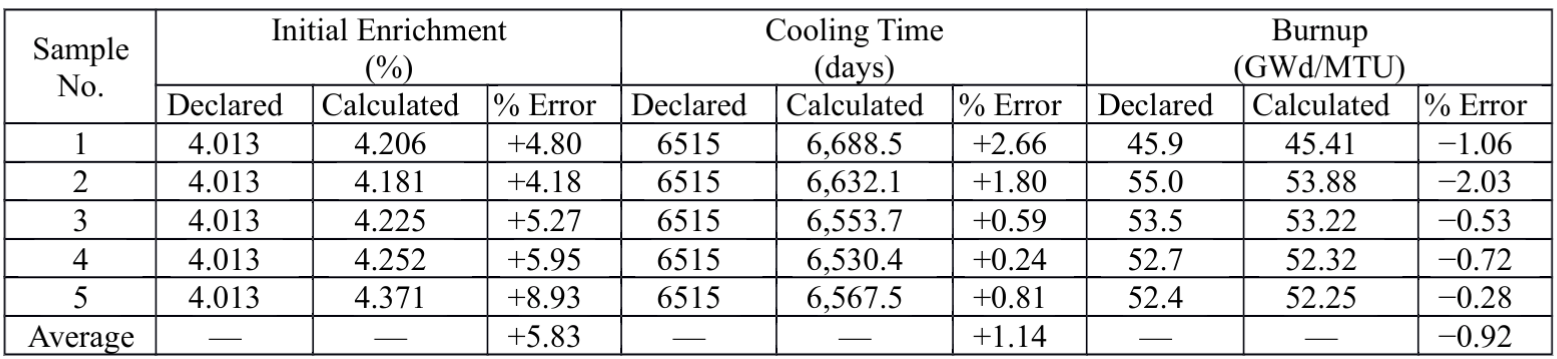
\includegraphics[width=\linewidth]{./chapters/litrev/indepth.png}
  \caption[Example of results from \acrshort{INDEPTH}]
          {Example set of results from \acrshort{INDEPTH} solving the inverse 
           problem being described in this work in Reference 
           \cite{grogan_indepth_2018}.}
  \label{tbl:indepth}
\end{table}

Through a nonlinear least-squares regression algorithm, repeated runs of
\gls{ORIGEN-ARP} are carried out given an initial guess. The squared error
residual is calculated from comparing the computed nuclide measurements against
a set of known nuclide measurements, and the repetition terminates when the sum
of the squared error is at some minimum.  \cite{weber_2006} This approach was
also tested with fission product measurements \cite{weber_2010} and later with
gamma spectra \cite{weber_2011}. Table \ref{tbl:indepth} shows an example of
the results from a set of samples that have the same \gls{U235} enrichment and
time since irradiation but different burnups.  The average error for the
enrichment is 5.83\%, but the other two parameters are both predicted within
approximately 1\% error. 

The iterative forward modeling approach has much merit, but another approach is
to use statistical methods to determine relationships between nuclide
measurements and reactor operation parameters. The background for this is
introduced next in Section \ref{sec:mlback} and discussed within the context of
nuclear forensics in Section \ref{sec:stats4nf}.

%Further, including measurement uncertainties broadens the linear model to
%probability densities of the parameters. The opposite is also true in the
%forward case: including parameter uncertainties broadens the forward problem
%results to probability densities of the potential measurement values.
%\cite{inverse_theory}
%
%In this way, we can define some probability that an answer is correct, given a
%set of measurements and their uncertainties, the calculated model parameters,
%the spread of the data space, and the spread of the model space. Inverse
%problem theory connects these values to the general form of Bayes' theorem,
%which is commonly expressed as follows:
%\begin{equation}
%  \label{eq:bayes}
%  P(A|B) = \frac{P(B|A)P(A)}{P(B)}
%\end{equation}

%Here, $A$ and $B$ are events, $P(A)$ and $P(B)$ are the probabilities that
%events $A$ and $B$ will occur, representing the model and data spaces,
%respectively. $P(A)$ is known as the likelihood and $P(B)$ is known as the
%marginal likelihood. The marginal likelihood is a concept of the data space
%capturing all the possible measurement values. It is ignored here because as a
%homogenous probability, it is only useful for determining absolute
%probabilities and this will only be applied in a relative context.  $P(B|A)$ is
%the prior probability that event $B$ will occur given a known result for $A$,
%which are the measurements given the model parameters (i.e. the forward
%problem).  $P(A|B)$ is the posterior probability that event $A$ will occur
%given a known result for $B$, which are the predicted model parameters given
%the measurements (i.e., the inverse problem) \cite{inverse_theory,
%gentle_bayes}. 

%This is can be mapped easily to the inverse physical system problem scenario.
%$A$ would represent an occurrence of a parameter in the model space, and $B$
%would represent the measurement of some value. Thus, $P(A)$ is the probability
%of a parameter existing without any knowledge of $B$. This is known as the
%prior probability, usually given by some theory about the system. $P(B)$ is the
%probability of some measurement existing without any knowledge of $A$. This is
%known as the marginal likelihood, which is some homogeneous concept for the
%potential measurements that could be made (this only serves to scale to
%absolute probabilities and does not affect the relative probabilities). The
%likelihood, $P(B|A)$, is the chance that a measurement is observed from a given
%parameter, representing the forward problem.  Lastly, the posterior probability
%is the chance of some parameter existing given some measurement, representing
%the inverse problem solution \cite{inverse_theory, gentle_bayes}.  
%
%Given the above, it is more intuitive to consider the conceptual version of
%Bayes' theorem in Equation \ref{eq:bayes_words}.
%\begin{equation}
%  \label{eq:bayes_words}
%  \text{Posterior} = \frac{\text{Likelihood} \cdot \text{Prior}}
%                          {\text{Marginal \ Likelihood}} 
%\end{equation} 
%
%This framework is helpful for an experiment that intends to compare different
%methods for calculating the posterior probability of a system given some
%measurements \cite{bayes_compare}.  In the nuclear forensics context of
%pre-detonated materials, this would be a a set of probabilities for different
%parameters of interest, e.g., reactor type, burnup, cooling time, and
%enrichment of some interdicted \gls{SNF}.

%In addition to evaluating a single learned model, it is beneficial to compare
%models. Moreover, there are potential degeneracies in the solution space. This
%is because most inverse problems are \textit{ill-posed}, because the solution
%is not guaranteed to be unique \cite{skutnik_2016}.  Evaluating not only the
%solution, but the confidence in the solution, is therefore prudent. While the
%two scikit-implemented algorithms do not provide this information, the
%\gls{MLL} calculation method provides a likelihood with an uncertainty. This
%provides a measure of distinguishability that many machine learning approaches
%do not provide. 

